\documentclass[12pt]{article}
\usepackage[hmargin=2.0cm,vmargin=1cm]{geometry}
\usepackage[utf8]{inputenc}
\usepackage{graphicx}
\usepackage{float}
\usepackage{cite}
\usepackage{natbib}
\usepackage{amsmath}

\title{\begin{LARGE}
{The environmental effect on LAEs galaxies at the end of reionization}
\end{LARGE}}

\begin{document}
\maketitle

%\section{Constants:}

%In this section we define the constants used in this work.

%\begin{table}[H]
%\begin{center}
%\begin{tabular}{c c c c}
%\hline
%Constant name & Symbol & Value & Units \\
%\hline
%\hline
%Boltzmann  & $k_B$ & $1.3806488\times 10^-{23}$ & $[J/K]$ \\ 
%Gravitational & $G$ & $6.67384\times 10^{-11}$ & $[\dfrac{m^3}{Kgs^2}]$\\
%Mean molecular weight &$\mu_n$ & $0.59$ & $-$ \\
%Proton mass & $m_p$ & $1.672621777\times 10^{-27}$ & [kg] \\
%Slope parameter & $\beta$ & $0.4$ & $-$ \\
%Matter density & $\Omega_m$ & $0.3089$ & $-$ \\ 
%Barions density & $\Omega_B$ & $ 0.0455102$ & $-$ \\
%Dark energy density & $\Omega_{\Lambda}$ & $0.6911$ & $-$ \\
%Spatial curvature density& $\Omega_{k} $ & $-0.0023$ & $-$ \\
%Hubble parameter & $H_0$ & $7.11449538303\times 10^{-41}$& $[1/s]$ \\
%Solar mass &  $M_{\odot} $ & $1.9891\times 10^{30}$  & [kg] \\ 
%$m_p$
%\hline
%\end{tabular}
%\end{center}
%\end{table}

\section{Gas density profile:}\label{sec:rho}

Makino et al (1997) found an analytical expresion (Eq.8 in that paper) for the gas profile assuming that the gas
is isothermal and it is inside a DM halo with a NFW profile. They argue that this equation it's well approximated by 
the following profile:

\begin{equation}\label{eq:rhogr}
\rho_g(r) =  \dfrac{\rho_{g,0}A}{\left[ 1 + \left(\dfrac{r}{r_{c,eff}}\right)^2 \right]^{3\beta_{eff}/2}}
\end{equation}

Where $A(b) = -0.178b + 0.982$ and $\beta_{eff} = 0.9 b$\\

In order to compute $\rho_{g,0}$ we used Eq.14 in that paper:

\begin{equation}\label{eq:rhog0}
\rho_{g0} = \dfrac{f_{gas}\Omega_{b}\rho_{c0}\delta_{c}}{\Omega_0}e^{27b/2} \left [ Ln(1+c) - \dfrac{c}{1+c}  \right ] \left [ \int_0^c x^2(1+x)^{27b/2x} dx \right ]
\end{equation}

As an example for a dark matter halo of $M_{vir} = 1E12 M_{\odot}$ at
$z=2$ with $c=3.75$. $\rho_{g,0}=1.37\times10^{-25} g/cm^{-3}$. The
density profile is shown in Fig. \ref{fig:gp}

\begin{figure}
\centering
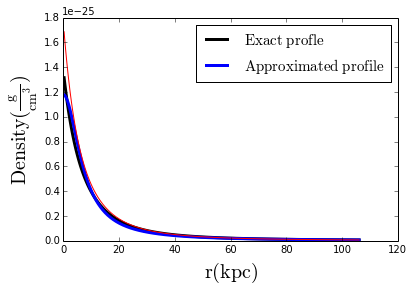
\includegraphics[scale=0.7]{../figures/gasprofile.png}
\caption{Gas density profile for a DM halo of $M_{vir} = 1E12
M_{\odot}$ at $z=2$ with $c=3.75$ \label{fig:gp}}
\end{figure}.


\section{Column density derivation:}\label{sec:NH}

The column density $N_{H}$ of the gas is:

\begin{equation}
N_{H} = \int \limits_{-\infty}^{\infty}\rho_g(r)dz
\end{equation}

Where $r^2 = z^2 + b'^2$ and $b'$ is the impact parameter (here z
should not be confused with the redshift).
Which in terms of $r$ is:

\begin{equation}
N_{H} = \rho_{g0}A \int \limits_{-\infty}^{\infty} \dfrac{dz}{\left
[ 1 + \left(\dfrac{r}{r_{c,eff}} \right)^2 \right]^{3\beta_{eff}/2}}
= \rho_{g0}A \int \limits_{b}^{\infty}\dfrac{r}{\sqrt{r^2 - b'^2}}\dfrac{dr}
{\left [ 1 + \left(\dfrac{r}{r_{c,eff}} \right)^2 \right]^{3\beta_{eff}/2}}
\end{equation}

The result of the integral is:

\begin{equation}\label{eq:NH}
N_{H} = \rho_{g0} A\dfrac{\sqrt{\pi} (\dfrac{1}{r_c(M_h)^2})^{-3\beta_{eff}(M_h) /2} (b'^2 + r_c(M_h)^2)^{1/2 - 3\beta_{eff}(M_h)/2} \Gamma(-1/2 + 3\beta_{eff}/2) }{2 \Gamma(\dfrac{3\beta_{eff}(M_h)}{2})}
\end{equation}


Figure \ref{fig:NHb} shows the dependence of the column density $N_H$
for different impact parameters $b'$ and different halo concentration.
\begin{figure}[H]
\centering
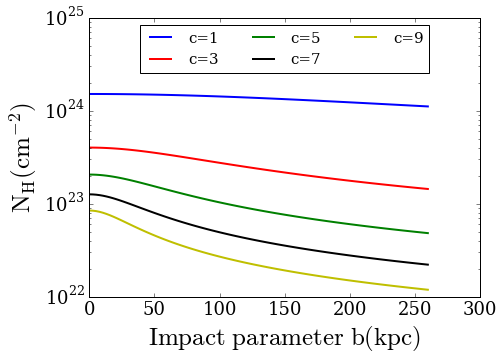
\includegraphics[scale=0.7]{../code/env/NH-b.png}
\caption{Column density values for different values of the impact
parameter and for different halo concentrations.\label{fig:NHb}}
\end{figure}

%The average column density $N_H$ of all the halos at all the possible
%impact parameters is:

%\begin{equation}\label{eq:integral}
%<N_H> = 4 \int \limits_0^{0.5} dx \int \limits_{0}^{0.5}dy \int
%\limits_{M_{Hmin}}^{M_{Hmax}} N_H(b, M_H)\xi(M_H)dM_H
%\end{equation}

%Where the impact paremeter $b'^2 = x^2  + y^2$ and $M_{Hmin} = 1\times 10^4
%M_{\odot}$ and $M_{Hmax} = 1\times 10^{12}M_{\odot}$. And $\xi(M_H)= \dfrac{dn}
%{dM_H}$. The dependence with the redshift is in the computation of $r_{vir}$ and
%in the mass function.

%To evaluate Eq.\ref{eq:integral} the integral over
%the mass using the trapezoid method is made:

%\begin{equation}
%\int \limits_{M_{HMin}}^{M_{HMax}} N_H(b, M_H)\xi(M_H)dM_H =  \sum_{0}^{1000}\Delta_M \left[ \dfrac{N_H(b, M_{H}+\Delta_M) \xi(M_{H + \Delta_M}) + N_H(b, M_{HM}\xi(M_{H}))}{2}\right]
%\end{equation}

%Which can be expressed as:

%\begin{equation}
%\begin{split}
%\int \limits_{M_{HMin}}^{M_{HMax}} N_H(b, M_H)\xi(M_H)dM_H = \sum \limits_{0}^{1000}\Delta_{M} M_{\odot}  \dfrac{\rho_{g0} A(b) \sqrt{\pi} \Gamma(-\dfrac{1}{2} + \dfrac{3\beta}{2})}{4\Gamma{\dfrac{3\beta}{2}}} \\
%\left[ \left( \dfrac{1}{r_c(M_{HMin})^2} \right)^{-3\beta/2} (b^2 + r_c(M_{Hmin})^2)^{1/2 - 3\beta/2} \xi(M_{Hmax})+ \\
% \left( \dfrac{1}{r_c(M_{HMax})^2} \right)^{-3\beta/2}(b^2 +r_c(M_{Hmax})^2)^{1/2 - 3\beta/2}\xi(M_{Hmin}) \right]
%\end{split}
%\end{equation}

%The average column density of a ray traced in a volume of $1Mpc^3$ at redshift $z=6$ is then given by:

%\begin{equation}
%<N_H> = 4 \rho_{g,0}A\int \limits_0^{0.5} dx \int \limits_{0}^{0.5}dy N_H(b) db = 1.68\times 10^{-42} \dfrac{g}{cm^3}
%\end{equation}


\section{Neutral Hydrogen fraction $\eta$:}\label{sec:eta}

To derive the neutral hydrogen fraction as a function of $n_H$ and the
temperature we follow Rahmati et al 2013. Here they assume ionization equilibrium.

The neutral hydrogen fraction $\eta = n_{HI} / n_H$
is defined as:\\

\begin{equation}\label{eq:eta}
\eta = \dfrac{B - \sqrt{B^2 - 4AC}}{2A}
\end{equation}

Where $A$ , $B$ and $C$ are defined as:

\begin{equation}
\begin{split}
A = \alpha_A + \Lambda_T \\
B = 2\alpha_A + \dfrac{\Gamma_{Phot}}{n_H} + \Lambda_T \\
C = \alpha_A
\end{split}
\end{equation}

Where $\Lambda_T$, $\alpha_A$ (Case A recombination rate) and
$\Gamma_{Phot}$ (Photoionization rate) are defined as:

\begin{equation}
\Lambda_T = 1.1.7 \times 10 ^{-10} \dfrac{T^{1/2} exp(-157809/T)}{1 + \sqrt(T/10^5)} cm^3 s^{-1}
\end{equation}


\begin{equation}
\alpha_A = 1.269 \times 10 ^{-13} \dfrac{\lambda^{1.503}}{(1 + (\lambda / 0.522)^{0.47} )^{1.923}} cm^{3} s^{-1}
\end{equation}

where $\lambda = 315614 / T$.

\begin{equation}
\Gamma_{Phot} = \Gamma_{UVB} \left(  0.98\left[ 1 + \left( \dfrac{n_H}{n_{H, SSh}} \right)^{1.64}  \right]^{-2.28} + 0.02 \left[ 1 + \dfrac{n_H}{n_{H,SSh}} \right]^{-0.84}   \right)
\end{equation}

Fig.\ref{fig:eta} shows the dependence of the neutral Hydrogen
fraction on the hydrogen density $n_H$ and temperature. Left panel
shows the dependence with $n_H$ for different Halo mass. Right panel
shows the dependence with temperature $T$, The blue
line is for a Hydrogen density $n_H = 0.01 cm^{-3}$
which is above the self-shielding density limit, while the black line is for $n_H  = 0.001 cm^{-3}$.

\begin{figure}[H]
\centering
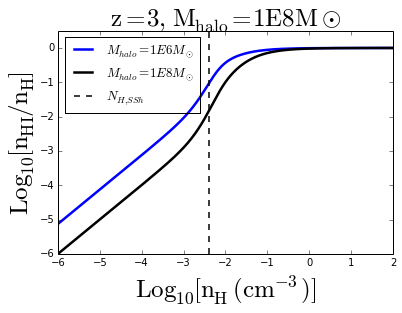
\includegraphics[scale=0.5]{../code/etavsnh.png}
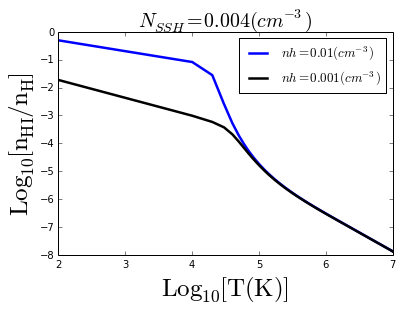
\includegraphics[scale=0.5]{../code/etavsT.png}
\caption{(Up)\label{fig:eta}}
\end{figure}

\section{Neutral Hydrogen density profile}\label{sec:NHI}

In order to study the effect of the environment on LAEs we are
interested in the neutral Hydrogen column density.
To this aim we want to derive the neutral Hydrogen gas profile using Makino's profile
alongside the neutral hydrogen fraction derived in the previous section.

As an example we made this for a Halo of mass $M_{vir} = 1 \times
10^{12} M_{\odot}$ at $z=2$ with $r_{vir}=106kpc$ and $T =2.4\times10^{6}K$.
Left panel in figure\ref{fig:nhvsr} shows the Hydrogen density $n_H$ derived from the density $\rho$
($n_H = \rho / m_p$). The neutral hydrogen fraction $\eta$ is shown in
the middle panel. While the neutral Hydrogen profile is shown in panel
right.

\begin{figure}[H]
\centering
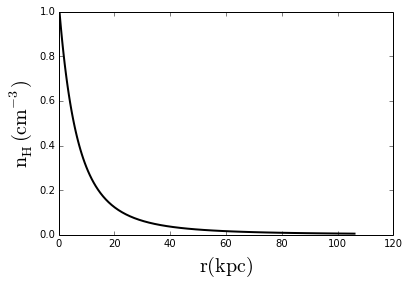
\includegraphics[scale=0.4]{../code/nhvsr.png}
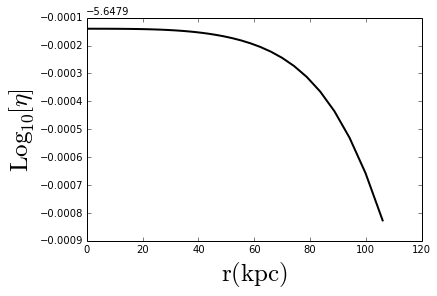
\includegraphics[scale=0.4]{../code/etavsr.png}
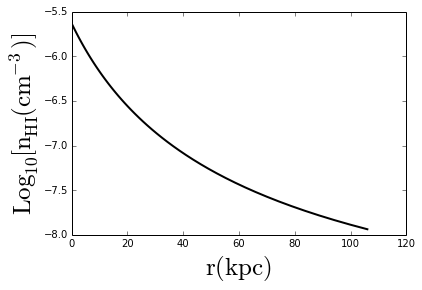
\includegraphics[scale=0.4]{../code/nhivsr.png}
\caption{\label{fig:nhvsr}}
\end{figure}

\section{Numerical Approach}

We use the results of the Dark Matter only simulation Illustris with the aim
of studying how the environment affects the absorption of
Ly$\alpha$ radiation at $z\sim6$. We chose emitters halos to be
those in a range of mass  $7 \times 10^{10} - 2 \times 10^{11}$, this
halos have different environments (\textbf{Make a plot of this}).

We then trace rays of Ly$\alpha$ photons in random directions, and we derive
the gas properties of those halos that interact with the ray
implementing the equations described in \S \ref{sec:rho},
\S \ref{sec:NH},\S \ref{sec:eta}.\S \ref{sec:NHI}. Then we sum the column
density of every Ly$\alpha$ ray. In the following subsections we describe
these steps in detail.

\subsection{Dark Matter halo catalogue}

We use the public available data from the Illustris simulation, in particular we use
the Illustis1-dark catalogue. This is a simulation of $1820^3$ dark matter particles
with a mass of $m_{DM}=6.3 \times 10^6 M_{\odot}$ in a box of $L=106.5 Mpc$. We use
the data of halos at $z = 6.01$.

We select emitter galaxies in the range of $7 \times 10^{10} - 2 \times 10^{11}$.
There are 1672 halos in this mass range in the simulation. These halos
are in different environment, in order to quantify the environment we
define $\Delta_3$ as:

\begin{equation}
\Delta_3  = \bar{r}^3 \left( \dfrac{1}{r^3} - \dfrac{1}{\bar{r}^3} \right)
\end{equation}

If $\Delta_3 < 0 $ the halo is in an over-dense environment while
if $\Delta_3 > 0 $ the halo is in an under-dense environment.

Left panel of figure \ref{fig:HalosEnv} shows the distribution of
halo mass, the color shaded are corresponds to the emitters halo mass
distribution. Right panel shows the halo mass against the
environment parameter $\Delta_3$.

\subsection{Ray tracing}

After selecting randomly an emitter we follow the trajectory of a Ly$\alpha$ photon
in a random direction and for ray length of $10 Mpc$. In $10 Mpc$ a Ly$\alpha$ would
have a $\Delta_z$ of:


We then compute the impact parameter $b$ between the ray and all the halos that could
possibly absorb the photons, we select those halos in which the condition $b<R_{vir}$
is ensured, those halos would be the absorbers.



\textbf{How many absorbers have each ray, try to visualize this}

\subsection{Column density properties and Environment}

We compute the density profiles of using Eq.\ref{eq:rhogr}, the
we compute the column density using Eq.\ref{eq:NH}. Then we compute
the fraction of neutral column density $n_{HI}$ using Eq.\ref{eq:eta}



\section{Results}


\end{document}
